\section{Modeling Process}
\label{sec:modeling} 

\textcolor{red}{Decision Tree}

For Yelp rating prediction, we use Decision Tree, which is tree-like graph of decisions and their possible consequences. It is widely used prediction model in machine learning. In this tree structure, leaves represent class labels and branches represent conjunctions of features that lead to the class labels. A typical example is shown in Figure \ref{fig:DT} \footnote{\url{https://en.wikipedia.org/wiki/Decision_tree_learning}}. The modeling process include feature selection, best split and tree generation. 

%-------------------------------------------
\begin{figure}[h]
	\centering
	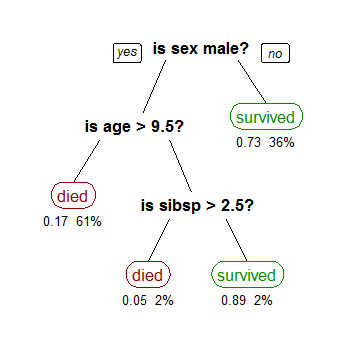
\includegraphics[width=5cm]{DT.png}
	\caption{A Decision Tree showing survivals of passengers of the Titanic.}
	\label{fig:DT}
\end{figure}
%------------------------------------------- 

\paragraph{Feature Selection}
There are multiple features related a user's rating. \textcolor{red}{give list or table, showing all features. }

\paragraph{Best Split}
Decision Tree works in a top-down manner, we need to choose a variable at each step that best split the sets of items. The best split are chosen by certain metric, e.g., Gini impurity, Information gain and so on. 

\paragraph{Tree Generation}
With the selected features, and variables chosen by best split, a tree can be generated. And each path in the tree represents a decision-making process, in which a user's rating can be predicted based on a series of decision makings. 